\chapter{Design}

\section{Introduction}
This chapter aims to provide a detailed overview of the software architecture and database design of the project. It is essential for understanding the organization and structure of the system, as well as the design choices made to ensure the efficiency, scalability, and robustness of the software.

The design of the software architecture focuses on the organization and distribution of software components, defining roles, responsibilities, and interactions among them. Key architectural decisions guiding the project's development will be presented within this context.

Additionally, the database design will be examined, with particular attention to the decision to use a NoSQL database like MongoDB. This decision was motivated by the need to adapt to the specific requirements of the project, including flexible management of unstructured data and horizontal scalability.


\section{Software Architecture}

\begin{figure}[ht!]
    \centering
    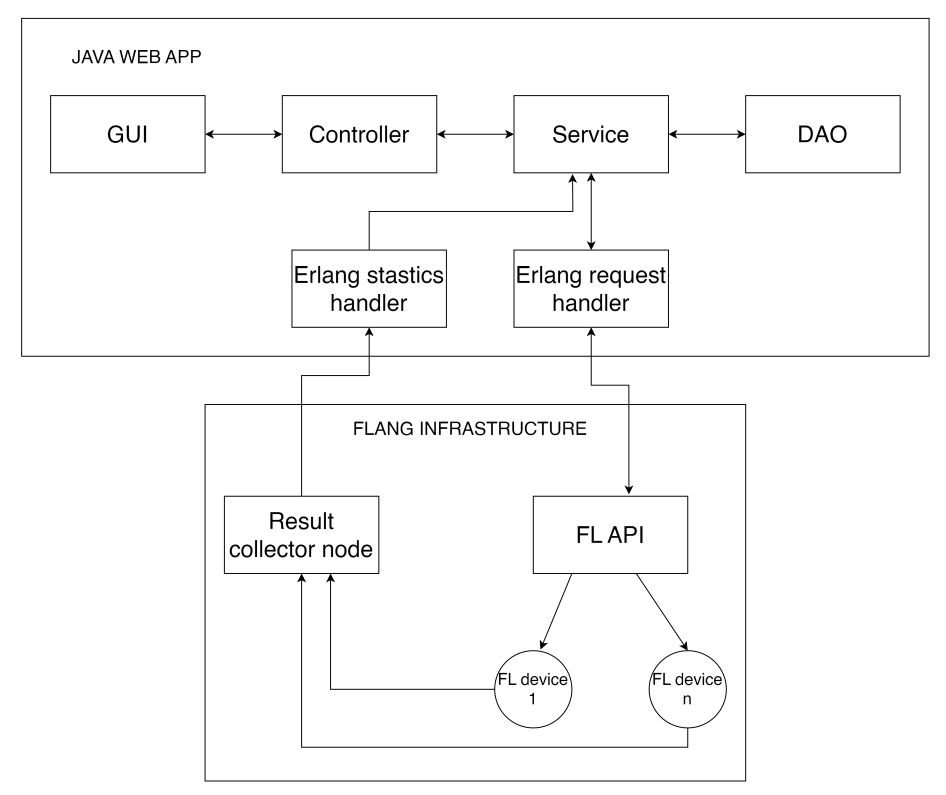
\includegraphics[width=0.8\textwidth]{images/2_analisys/FL_proj_Arch..png}
    \caption{System Architecture}
    \label{fig:system_architecture}
\end{figure}


\newpage
\section{Database Design}

\subsection{MongoDB}
\subsubsection{Collections}
\textbf{ExpConfig document example:} \begin{verbatim}
        {
            "id": "example_id",
            "name": "Example Experiment",
            "algorithm": "example_algorithm",
            "strategy": "example_strategy",
            "numClients": 10,
            "stopCondition": "example_condition",
            "threshold": 0.5,
            "parameters": {
                "param1": "value1",
                "param2": "value2",
                "param3": "value3"
            },
            "creationDate": "2024-03-14T00:00:00Z",
            "lastUpdate": "2024-03-14T12:00:00Z"
        }
    \end{verbatim}
\textbf{Experiment document example:} \begin{verbatim}
        {
            "id": "example_id",
            "name": "Example Experiment",
            "expConfigSummary": {
                "id": "exp_config_id",
                "name": "Example Configuration",
                "algorithm": "example_algorithm"
            },
            "creationDate": "2024-03-14T00:00:00Z",
            "lastUpdate": "2024-03-14T12:00:00Z",
            "status": "Completed"
        }
    \end{verbatim}

    \textbf{ExperimentMetrics document example:} \begin{verbatim}
        {
            "id": "id",
            "expId": "exp_id",
            "type": "type",
            "hostMetrics": {
                "cpuUsage": 15.5,
                "memoryUsage": 65,
            },
            "modelMetrics": {
                "FRO": 0.154,
                "F1": 0.654,
            },
            "Timestamp": "2024-03-14T00:00:00Z",
            "expStatus": "running"
        }
    \end{verbatim}

\newpage
\textbf{User document example:} \begin{verbatim}
        {
        "id": "example_user_id",
        "email": "user@example.com",
        "password": "example_password",
        "creationDate": "2024-03-14T00:00:00Z",
        "configurations": ["config_id1", "config_id2"],
        "experiments": [
            {
            "id": "experiment_summary_id1",
            "name": "Experiment 1",
            "configName": "Configuration 1",
            "creationDate": "2024-03-14T06:00:00Z",
            },
            {
            "id": "experiment_summary_id2",
            "name": "Experiment 2",
            "configName": "Configuration 2",
            "creationDate": "2024-03-14T09:00:00Z",
            "lastUpdate": "2024-03-14T12:00:00Z"
            }
        ],
        "role": "example_role"
    }

    \end{verbatim}
\newpage
\section{Message Handler}

\subsection{Erlang for Message Passing}
The message handler is implemented using the Erlang programming language. Erlang is a functional programming language designed for building scalable and fault-tolerant systems. It is particularly well-suited for building distributed systems, thanks to its lightweight processes and built-in support for message passing. In this project, it's utilized the Jinterface library, which allows to write Java code that can communicate with Erlang processes to send and receive messages, arriving from the FLang Infrastructure and vice versa.

\subsection{Message Structure}
\begin{itemize}
    \item Error Message:
    \begin{verbatim}
        {
            "type": "error",
            "cause": "error_in_collecting_data",
            "timestamp": "2024-03-13T12:34:56"
        }
    \end{verbatim}
    
    \item Stop Message:
    \begin{verbatim}
        {
            "type": "stop",
            "cause": "experiment_finished",
            "timestamp": "2024-03-13T12:34:56"
        }
    \end{verbatim}
    
    \item Data Message:
    \begin{verbatim}
        {
            "type": "data",
            "parameters": {
                "param1": "value1",
                "param2": "value2"
            },
            "timestamp": "2024-03-13T12:34:56",
            "status": "running"
        }
    \end{verbatim}
\end{itemize}

\subsection{Description of the Erlang Message Handler Module}
The Erlang message handler module is a crucial component of the system responsible for managing incoming messages, processing them accordingly, and facilitating communication between different parts of the distributed system. It encapsulates the logic for handling various types of messages, such as error notifications, stop signals, and data updates, ensuring proper routing and processing. Additionally, the module provides interfaces for sending and receiving messages, abstracting the underlying communication mechanisms and enabling seamless integration with other system components. Its robust design and fault-tolerant features contribute to the overall reliability and performance of the distributed system.